\documentclass[a4paper, 11pt]{article}

\usepackage{fullpage}

\usepackage[english,russian]{babel}
\usepackage[utf8]{inputenc}
\usepackage{amsmath, amsfonts, amssymb, amsthm}
\usepackage{mathtools}
\usepackage{bm}

\usepackage{hyperref}
\usepackage{booktabs}
\usepackage{graphicx}
\usepackage{subcaption}

\usepackage[linesnumbered,ruled,vlined]{algorithm2e}
\SetKwInput{KwInput}{input}
\SetAlFnt{\small}

\usepackage{float}

\newtheorem{definition}{Определение}
\newtheorem{theorem}{Теорема}
\newtheorem{lemma}{Лемма}

\begin{document}

\begin{titlepage}
	\newpage
	
	\begin{center}
		%	Московский Государственный Университет им. М. В. Ломоносова \\
	\end{center}
	
	\vspace{8em}
	
	\begin{center}
		%\Large Кафедра Вычислительных Технологий и Моделирования \\ 
	\end{center}
	
	\vspace{2em}
	
	\begin{center}
		\textsc{\textbf{Метод конечных объемов: теоретические сведения и программная реализация}}
	\end{center}
	
	\vspace{6em}
	
	
	
	\newbox{\lbox}
	\savebox{\lbox}{\hbox{}}
	\newlength{\maxl}
	\setlength{\maxl}{\wd\lbox}
	\hfill\parbox{11cm}{
		%\hspace*{5cm}\hspace*{-5cm}Студент:\hfill\hbox {Иванов И. И.\hfill}\\
		%\hspace*{5cm}\hspace*{-5cm}Преподаватель:\hfill\hbox {Ануприенко Д. В.\hfill}\\
		%	\\
		%\hspace*{5cm}\hspace*{-5cm}Группа:\hfill\hbox {403}\\
	}
	
	
	\vspace{\fill}
	
	\begin{center}
		Москва \\ 2022
	\end{center}
	
\end{titlepage}

\setcounter{MaxMatrixCols}{20}

\section{Общие сведения о методе конечных объемов}

Метод конечных объемов (МКО, также метод контрольного объема, метод баланса, интегро-интерполяционный метод) наряду с рассмотренными ранее методами конечных разностей (МКР) и конечных элементов (МКЭ) является способом преобразования задачи для уравнения в частных производных в систему алгебраических уравнений для сеточных неизвестных. 

В отличие от МКЭ, имеющего обширную математическую базу, МКО строится на более физических принципах. Хотя это затрудняет математический анализ метода, получающаяся численная схема обладает рядом преимуществ, среди которых \textit{консервативность}. Консервативность схемы означает, что полученное численное решение удовлетворяет некоторым законам сохранения, которым удовлетворяет решение исходной задачи. В методе конечных объемов это свойство выполняется на каждой ячейке.

\section{Построение метода конечных объемов}
\subsection{Построение консервативной разностной схемы для одномерного уравнения диффузии}
Рассмотрим краевую задачу для одномерного стационарного уравнения диффузии:
\begin{equation}
\begin{cases}
-\frac{\partial}{\partial x} \left(D\frac{\partial C}{\partial x}\right) = s~~\text{в}~~\Omega=\left(0;1\right),\\
C\left(0\right) = a,~~C\left(1\right)=b.
\end{cases}
\end{equation}

Считаем пока коэффициент диффузии $D$ постоянным. 
Рассмотрим для удобства уравнение в смешанной форме:
\begin{equation}\label{eq:diff_1d_mixed}
\begin{cases}
\frac{\partial q}{\partial x} = s~~\text{в}~~\Omega=\left(0;1\right),\\
q = -D\frac{\partial C}{\partial x},\\
C\left(0\right) = a,~~C\left(1\right)=b.
\end{cases}
\end{equation}

Введем равномерную сетку на отрезке $(0;1)$ с шагом $\Delta x = 1/N$. На сей раз неизвестные расположим, в отличие от МКР и МКЭ, не в узлах, а в центрах ячеек сетки (пример для $N = 4$ приведен на рисунке \ref{pic:fvm_1d}). На этой сетке определим ячейки $e_i=\left[x_i;~x_{i+1}\right]$. Координата центра $i$-й ячейки обозначается как $x_{i+1/2}$.

\begin{figure}[h] \centering
	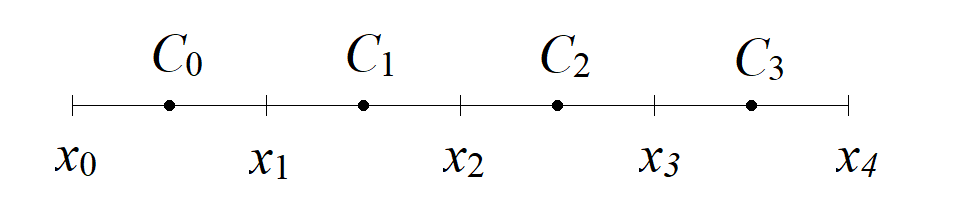
\includegraphics[scale=0.4]{fvm_1d}
	\caption{Одномерная сетка и расположение сеточных значений концентрации в центрах ячеек\label{pic:fvm_1d}}
\end{figure}

Далее проинтегрируем закон сохранения массы (первое уравнение в \eqref{eq:diff_1d_mixed}) по ячейке $e_i$:
\begin{equation}
\int_{e_i}
\frac{\partial q}{\partial x}dx = \int_{e_i}sdx,
\end{equation}
из которого получим
\begin{equation}\label{eq:fvm_1d_masscons}
q_{i+1} - q_i = \int_{e_i}sdx,
\end{equation}
где $q_i$ -- поток в узле $i$. 

Перейдем теперь к выражению для потока (второму уравнению в  \eqref{eq:diff_1d_mixed}). Для внутренних узлов поток выражается просто:
\begin{equation}
q_i = -D\frac{C_i - C_{i-1}}{\Delta x},
\end{equation}

Для граничных же узлов эти выражения несколько меняются
\begin{equation}
q_0 = -D\frac{C_0 - a}{\Delta x /2},~~q_{N-1} = -D\frac{b - C_{N-1}}{\Delta x/2}.
\end{equation}

Полученные выражения для потоков можно подставить в уравнения \eqref{eq:fvm_1d_masscons}. Для внутренних ячеек они принимают вид
\begin{equation}
-D\frac{C_{i+1} - C_{i}}{\Delta x} + D\frac{C_i - C_{i-1}}{\Delta x} = \int_{e_i}sdx.
\end{equation}
Если интеграл в правой части приблизить формулой $\int_{e_i}fdx \approx f(x_{i+1/2}) \cdot\Delta x$, а затем поделить все на $\Delta x$, получим
\begin{equation}
-D\frac{C_{i+1} - 2C_{i} + C_{i+1}}{\Delta x^2} = s(x_{i+1/2}).
\end{equation}
Уравнения для граничных ячеек отличаются несильно. Итоговая система имеет трехдиагональную матрицу и сильно похожа на дискретизацию традиционной разностной схемой с трехточечным шаблоном.

\subsection{Метод конечных объемов в двумерном случае}

Подобные действия можно проделать и в двумерном случае. Выпишем и здесь систему в смешанном виде:
\begin{equation}
\begin{cases}
\nabla\cdot\mathbf{q} = s~~\text{в}~~\Omega\in\mathbb{R}^2,\\
\mathbf{q} = - \mathbb{D}\nabla C,\\
+~\text{граничные условия}
\end{cases}
\end{equation}

Пусть $e_i$ -- некоторая ячейка сетки. Проинтегрируем закон сохранения массы по ячейке:
\begin{equation}
\int_{e_i}\nabla\cdot\mathbf{q}~dV = \int_{e_i}s~dV,
\end{equation}
затем левую часть преобразуем по теореме Остроградского--Гаусса:
\begin{equation}
\int_{e_i}\nabla\cdot\mathbf{q}~dV = \int_{\partial e_i}\mathbf{q}\cdot\mathbf{n}~dS,
\end{equation}
где $\mathbf{n}$ -- нормаль к границе $e_i$. На практике ячейка сетки является многоугольником, поэтому преобразование можно продолжать дальше:
\begin{equation}
\int_{e_i}\nabla\cdot\mathbf{q}~dV = \int_{\partial e_i}\mathbf{q}\cdot\mathbf{n}~dS 
= 
\sum_{f \in \partial e_i} \int_{f}\mathbf{q}\cdot\mathbf{n} ~dS
\end{equation}

Здесь $f$ -- грань ячейки; используется терминология, более привычная для трехмерного варианта МКО. В двумерном случае для ячейки грань = ребро, а в INMOST для двумерных ячеек Face и Edge являются одним и тем же понятием.

Ключевым вопросом при построении схемы МКО является приближение интеграла $\mathbf{q}\cdot\mathbf{n}$ на грани -- \textit{интегрального потока через грань}. Далее для краткости будем говорить просто "потока через грань".

\section{Схема с двухточечной аппроксимацией потока через грань}

Эта схема является простейшим вариантом МКО, широко используемым на практике. В выражении для потока через грань используются значения концентрации только в двух точках -- центрах масс двух ячеек, разделяемых гранью (если грань внутренняя; а в случае граничной грани вместо центра масс отсутствующей ячейки используется значение концентрации в центре масс грани -- об этом далее). Поэтому схема и называется двухточечной (англ. two-point flux approximation, TPFA).

Далее рассмотрим построение аппроксимации для грани $f$, разделяющей ячейки $A$ и $B$ (см. рисунок \ref{pic:tpfa}). Используется следующее выражение:

\begin{equation}\label{eq:tpfa_idea}
%\mathbf{q}\cdot\mathbf{n}|_{\text{грань}} = 
\int_{f}\mathbf{q}\cdot\mathbf{n} ~dS
\approx
|f|\cdot t_f \cdot (C_B - C_A),
\end{equation}
где $|f|$ -- площадь грани (длина ребра), $C_A$, $C_B$ -- концентрации в центрах масс ячеек, $t_f$ -- коэффициент проводимости (англ. transmissibility). Как его искать?

\begin{figure}[h] \centering
	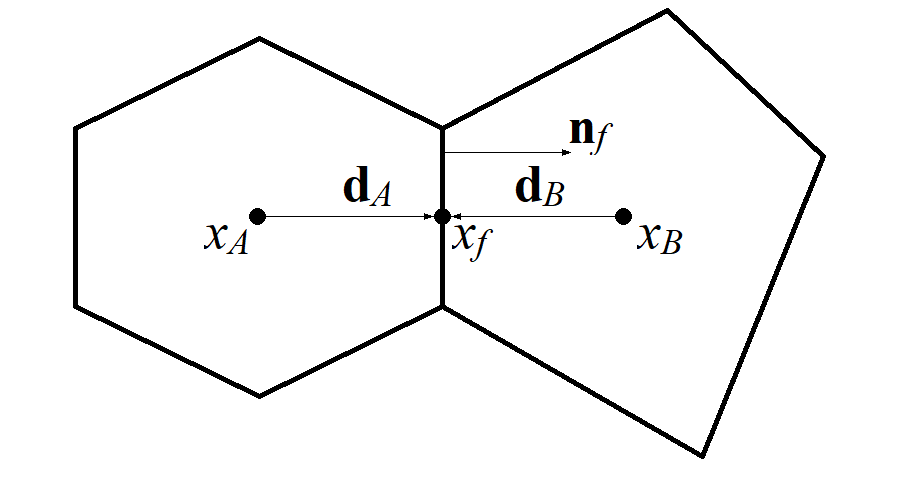
\includegraphics[scale=0.4]{fvm_tpfa}
	\caption{Две ячейки и необходимые для построения аппроксимации потока величины\label{pic:tpfa}}
\end{figure}

Для начала определим некоторые величины (все они приведены на рисунке \ref{pic:tpfa}):
\begin{itemize}
	\item $x_{A,B}$ -- центры масс ячеек;
	\item $x_f$ -- центр масс грани;
	\item $\mathbf{d}_{A,B} = \overrightarrow{x_{A,B}x_f}$ -- векторы, соединяющие центры масс ячеек и центр масс грани;
	\item $\mathbf{n}_f$ -- \textit{единичный} вектор нормали к грани, направленный \textit{из $A$ в $B$};
	\item $\mathbb{D}_{A,B}$ -- тензоры диффузии в ячейках, они могут отличаться.
\end{itemize}

Введем в центре масс грани $f$ вспомогательную величину -- концентрацию $C_f$. Далее построим с ее помощью выражения, аппроксимирующие поток для ячеек $A$ и $B$, затем их приравниванием эту неизвестную исключим. Начнем с аппроксимации градиента:

\begin{equation}
\left(\nabla C\right) _{A,B}
\approx
(C_f - C_{A,B}) \frac{\mathbf{d}_{A,B}}{||\mathbf{d}_{A,B}||^2}.
\end{equation}

Используя эти выражения, приблизим величину $\mathbf{q}\cdot \mathbf{n} = -\mathbb{D} \nabla C \cdot \mathbf{n}$:

\begin{equation}\label{eq:tpfa_subflux}
\left(
\mathbf{q}\cdot \mathbf{n}\right)_f
\approx
-(C_f - C_{A,B}) \frac{\mathbb{D}\mathbf{d}_{A,B}\cdot\mathbf{n}_f}{||\mathbf{d}_{A,B}||^2}.
\end{equation}

Далее, выписав отдельно выражения для двух ячеек, приравняем их, приведем неизвестные и выразим $C_f$. Проделать это можно в качестве практического задания. Итоговое выражение для потока через грань принимает вид

\begin{equation}
\left(
\mathbf{q}\cdot \mathbf{n}\right)_f
\approx
(C_B - C_A)
\frac
{
\frac{\mathbb{D}\mathbf{d}_A\cdot\mathbf{n}_f}{||\mathbf{d}_A||^2}
\cdot
\frac{\mathbb{D}\mathbf{d}_B\cdot\mathbf{n}_f}{||\mathbf{d}_B||^2}
}
{
\frac{\mathbb{D}\mathbf{d}_A\cdot\mathbf{n}_f}{||\mathbf{d}_A||^2}
-
\frac{\mathbb{D}\mathbf{d}_B\cdot\mathbf{n}_f}{||\mathbf{d}_B||^2}
}.
\end{equation}
Таким образом, для коэффициент проводимости равен
\begin{equation}\label{eq:tpfa_trans}
t_f = 
\frac
{
	\frac{\mathbb{D}\mathbf{d}_A\cdot\mathbf{n}_f}{||\mathbf{d}_A||^2}
	\cdot
	\frac{\mathbb{D}\mathbf{d}_B\cdot\mathbf{n}_f}{||\mathbf{d}_B||^2}
}
{
	\frac{\mathbb{D}\mathbf{d}_A\cdot\mathbf{n}_f}{||\mathbf{d}_A||^2}
	-
	\frac{\mathbb{D}\mathbf{d}_B\cdot\mathbf{n}_f}{||\mathbf{d}_B||^2}
}.
\end{equation}

\subsection{Обработка граничных условий}
В МКО граничные условия определяются \textit{на гранях}. Для каждой грани задается либо концентрация в центре масс, либо интегральный поток через эту грань. Таким образом, в случае граничного условия Неймана все тривиально: интегральный поток уже известен, и его можно просто отправить в правую часть итоговой линейной системы. 

Для условия Дирихле все тоже не очень сложно. Аппроксимация строится аналогично случаю внутренних граней, только отсутствует ячейка $B$, и для аппроксимации потока можно оставить выражение \eqref{eq:tpfa_subflux}.

\subsection{Детальный алгоритм сборки системы уравнений}
\begin{algorithm}
	\SetAlgoLined
	
	\For{$f \in $ все грани сетки}{
		Найти величины $\mathbf{n}_f$, $x_f$\;
		\eIf{$f$ -- граничная грань}{
			\eIf{$f$ -- грань Дирихле}{
				Определить соответствующую ячейку $A$\;
				Найти величины $x_A$, $\mathbf{d}_A$, $\mathbb{D}_A$\;
				Найти коэффициент в выражении \eqref{eq:tpfa_subflux}\;
				Добавить в линейную систему в строку, соотвествующую ячейке $A$, соответствующие элементы в матрицу и в правую часть (через <<+=>>, не через <<=>>!)\;
				Не забыть умножить на $|f|$\;
			}{
			В случае грани Неймана добавить в правую часть в строку, соотвествующую ячейке $A$, значение интегрального потока на грани.
		    }
		}{
			Для внутренней грани определить ячейки $A$ и $B$\;
			Найти величины $x_{A,B}$, $\mathbf{d}_{A,B}$, $\mathbb{D}_{A,B}$\;
			Вычислить проводимость $t_f$ в соответствии с \eqref{eq:tpfa_trans}\;
			В соответствии с \eqref{eq:tpfa_idea} (не забыть там $|f|$) добавить элементы в матрицу системы (всего 4 элемента, по 2 в строках для $A$ и $B$)\;
			Не забыть использовать <<+=>> вместо <<=>> при модификации матрицы.
		}
	}

\For{$c \in $ все ячейки сетки}{
	Найти центр масс ячейки $x_c$\;
	Добавить в правую часть элемент $s(x_c)\cdot |c|$\;
	Не забыть использовать <<+=>> вместо <<=>>\;
}
\end{algorithm}

Полезные функции INMOST, которые пригодятся здесь:
\begin{itemize}
	\item \texttt{Barycenter()} -- вычислить центр масс. Не путать с \texttt{Centroid()}, которая ищет центроид -- среднее арифметическое координат, что может не быть центром масс;
	\item \texttt{Face::UnitNormal()} -- найти единичную нормаль к грани;
	\item \texttt{Face::BackCell()} -- получить для грани ячейку, по отношению к которой нормаль является внешней (на рисунке \ref{pic:tpfa} -- ячейку $A$);
	\item \texttt{Face::FrontCell()} -- получить для грани ячейку, по отношению к которой нормаль является внутренней (на рисунке \ref{pic:tpfa} -- ячейку $B$). Не сработает для граничной грани;
	\item \texttt{rMatrix::FrobeniusNorm()} -- посчитать фробениусову норму матрицы, для матрицы-столбца выдаст обычную евклидову норму вектора;
	\item \texttt{Face::Area()} -- найти площадь грани (длину ребра);
	\item \texttt{Cell::Volume()} -- найти объем (площадь) ячейки.
\end{itemize}

\section{Что нужно запрограммировать}

Устройство кода похоже на код по МКЭ. Отличия следующие:

\begin{itemize}
	\item Значения концентраций (рассчитанной и аналитической) и источника находятся в ячейках, а не в узлах;
	\item Соответственно, тег глобальных индексов тоже должен быть определен на ячейках;
	\item Граничные условия задаются на гранях, а не в узлах;
	\item Наличие ГУ Дирихле не влияет на число неизвестных, оно всегда равно числу ячеек.
\end{itemize}
~\\
Дополнительно нужно сделать следующее:

\begin{itemize}
	\item Оценку $L_2-$ и $C-$норм ошибки, при этом воспользоваться старым заданием, где это проделывалось для кусочно-постоянных функций;
	\item Создать специальный тег, определенный на гранях, и записать туда проводимости $t_f$;
	\item С помощью этого тега затем можно вычислять потоки. Поскольку визуализировать данные на гранях мы не можем, будем хранить вектор потока на ячейках, вычисляя его для ячейки $e$ как
	\begin{equation*}
	\mathbf{q}|_e = \frac{1}{|e|}\sum_{f \in \partial e}\left(\mathbf{q}\cdot\mathbf{n}\right)|_f \cdot (x_f - x_e),
	\end{equation*}
	где значения $\left(\mathbf{q}\cdot\mathbf{n}\right)|_f $ находятся с использованием рассчитанных концентраций и проводимостей.
\end{itemize}

\section{Заключение}

Рассмотрен метод конечных объемов с простейшей двухточечной аппроксимацией интегрального потока через грани ячеек. В отличие от МКЭ, этот метод располагает неизвестные в ячейках, а не в узлах. Количество неизвестных не меняется в зависимости от граничных условий и всегда равно числу ячеек. Метод локально консервативен, по построению его в каждой ячейке выполняется закон сохранения массы, а двухточечная аппроксимация потока обладает рядом преимуществ -- компактный шаблон и удовлетворение дискретному принципу максимума, простота программирования. В чем же подводные камни? Ответ дадут численные эксперименты.

\end{document}